\subsection{Pruebas unitarias}
Las pruebas unitarias son una forma de comprobar que un fragmento de c�digo funciona correctamente.Son peque�os tests que validan el comportamiento de un objeto y la l�gica \citep{gutierrez2006pruebas}. \ac{xp} plantea la realizaci�n de pruebas unitarias continuas, frecuentemente repetidas y automatizadas, incluyendo pruebas de regresi�n, y aconseja escribir el c�digo de la prueba antes de la codificaci�n \citep{kniberg2007scrumyxp}.\\
Para la aplicaci�n de las pruebas unitarias a la soluci�n se emple� el framework JUnit el cual permite realizar la ejecuci�n de clases Java de manera controlada, para poder evaluar si el funcionamiento de cada uno de los m�todos de la clase se comporta como se espera. Es decir, en funci�n de alg�n valor de entrada se eval�a el valor de retorno esperado; si la clase cumple con la especificaci�n, entonces JUnit devolver� que el m�todo de la clase pas� exitosamente la prueba; en caso de que el valor esperado sea diferente al que regres� el m�todo durante la ejecuci�n, JUnit devolver� un fallo en el m�todo correspondiente.
\begin{figure}[h]
	\centering
	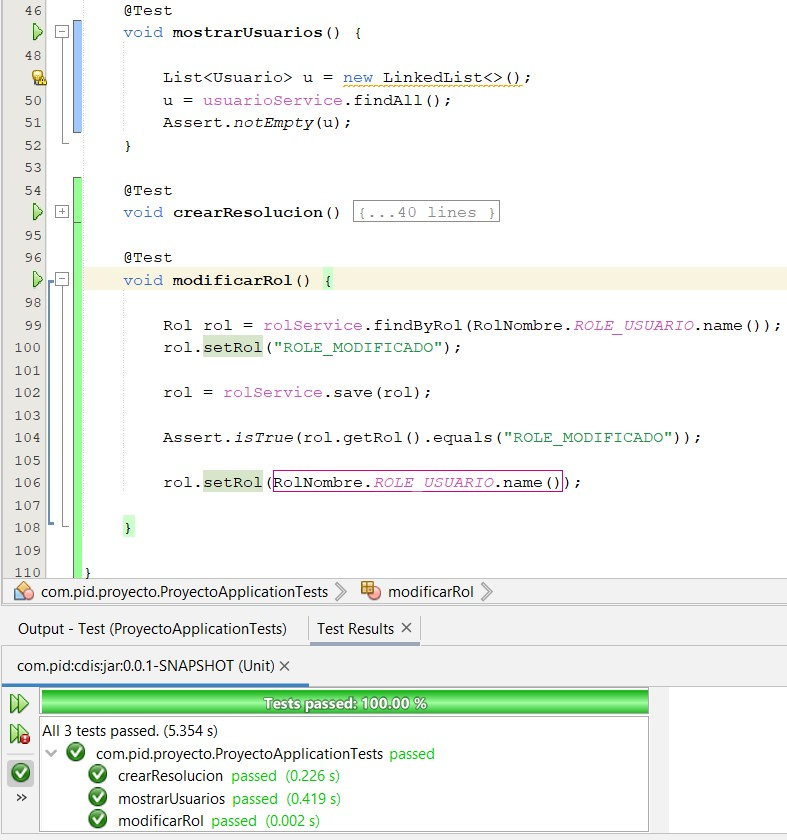
\includegraphics{images/test/unit-tests.jpg}
	\caption{Resultado de la ejecuci�n de pruebas unitarias en el c�digo fuente de CDIS.}
	\label{fig:unit-tests}
\end{figure}